\documentclass[../Master.tex]{subfiles}
\bibliography{../Bibliography}

\begin{document}
\afterpage{\blankpage}
\cleardoublepage

\chapter{Results and discussion}

\section{Pyrazole Ligand Development}\label{sec:pyr-dev}

\subsection{Starting Materials}\label{sec:starting-materials}

While several ligands were synthesized and utilized within the research group led by Professor L. Carlucci, my specific contribution focused exclusively on one of these ligands, that is based upon an already studied one. The structure of the starting material, 4,4’-malonyldibenzoic, and the retrosynthetic approch to it's reported in\ \ref{fig:dikest2-retro}.

\begin{figure}[h]
	\centering
	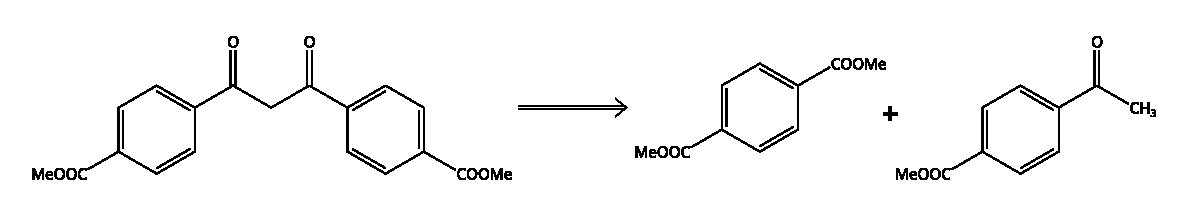
\includegraphics[width=16cm,height=8cm,keepaspectratio]{Structures/dikest2-retro.eps}
	\caption{4,4’-malonyldibenzoic acid Retrosynthesis Approach}\label{fig:dikest2-retro}
\end{figure}

The synthesis of the ligand is based on the cross-Claisen condensation followed by the hydrolisis of methylesters groups. The reaction was conducted with excellent yields and purity, resulting in the production of tens of grams of the compound. The reagents required for the synthesis are readily available commercially, facilitating the accessibility and reproducibility of the process. \\
The same synthetic approach has been carried out over a wide range of analogue compound, resulting tipically in high yield scalable reaction, as an example the ligand that will be analyzed in the section\ \ref{sec:electrochemistry} has been approached with the same strategies.\\
The detailed information on the synthesis and charactherization of 4,4’-malonyldibenzoic are reported in the section\ \ref{cha:experimental-section}.
\newpage
\subsection{Pyrazole Ligand Retrosynthesis}\label{sec:pyrazole-reaction}
Starting from the 1,3-diketone diester intermediate, obtained from the cross Claisen condensation, the apparently easier way to procede with the pyrazole formation is using hydrazine, of which a brief reaction mechanism is reported.

\begin{figure}[h!]
	\centering
	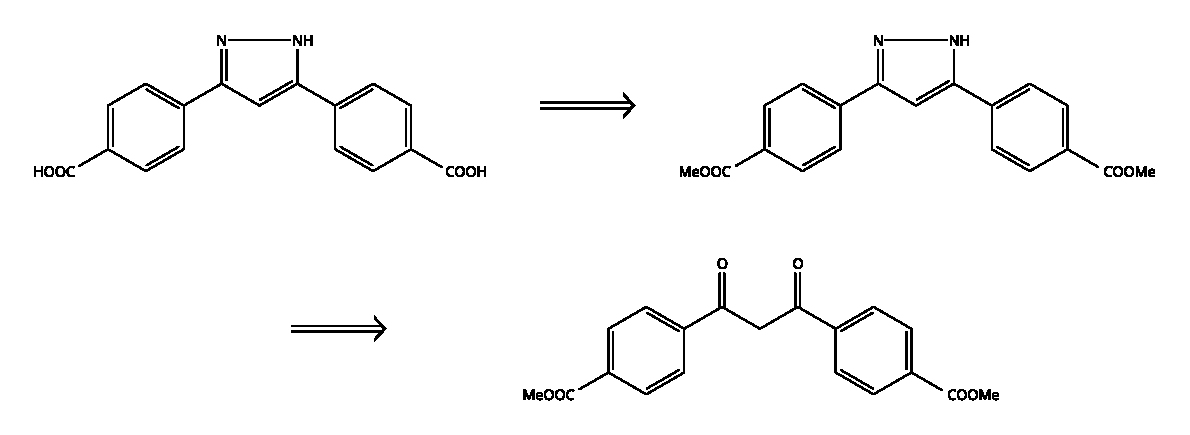
\includegraphics[width=16cm,height=8cm,keepaspectratio]{Structures/pyrazole-retro.eps}
	\caption{Pyrazole Ligand Retrosynthesis}\label{fig:pyrazole-retro}
\end{figure}

Typically, the reaction reaches completion in ethanol under reflux conditions with an excess of hydrazine within a few hours withouth any catalyzer: in this specific case several problems have been encountered and analyzed.\\

\begin{figure}[h!]
	\centering
	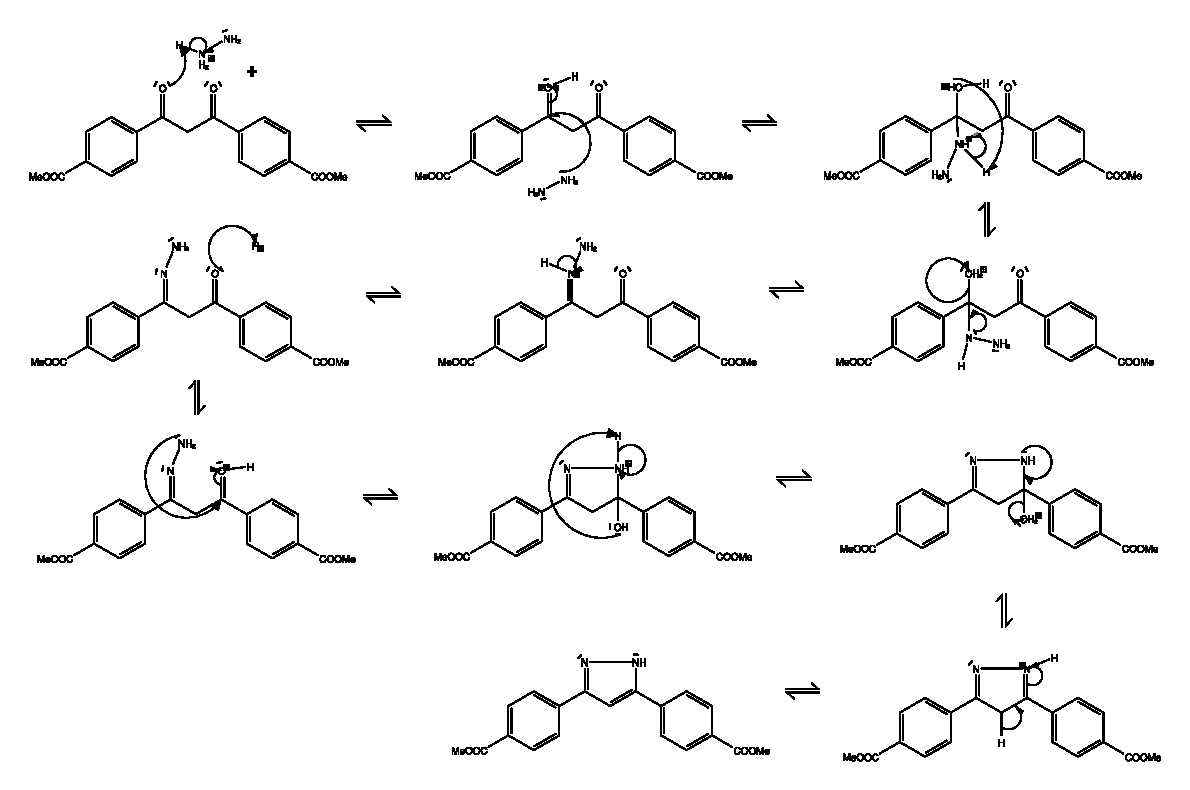
\includegraphics[width=15cm,keepaspectratio]{Structures/dikmecha.eps}
	\caption{Pyrazole Formation Mechanism}
\end{figure}

After hydrazine addition the diester intermediate must undergo hydrolisis to obtain the corrisponding dibenzoic acid. The conditions for this step have also been analyzed.

\subsection{Pyrazole Diester Formation}\label{sec:pyrazole-diester}

During the iterative process of analysing the reaction conditions, certain key characteristics of the starting reagents and the product of interest were crucial. The diketone intermediate possesses a characteristic straw-yellow colour, and also exhibits photoluminescence in the yellow-green range easily observed with a UV lamp. The pyrazole product is whitish and returns intense blue emission.\\
Numerous variables influencing the course of the reaction were evaluated, the results of which are given below. The use of IR spectroscopy and NMR structural analysis have been crucial in recognising the products formed, and also the mixtures left over from failed reactions, especially in the first attempts.

\begin{figure}[h!]
	\centering
	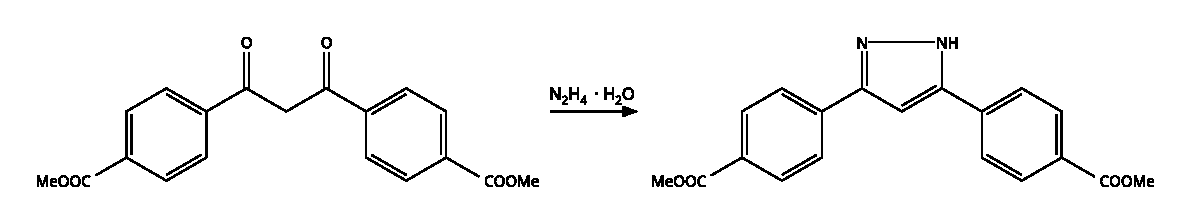
\includegraphics[width=13cm,height=8cm,keepaspectratio]{Structures/pyrazole-form.eps}
	\caption{Pyrazole Formation (solvent for the reaction are discussed below)}\label{fig:pyrazole-form}
\end{figure}

\subsubsection{Solvent Choice and Reagent Solubility}\label{sec:solvent}

Dimethyl 4,4’-malonyldibenzoate is poorly soluble in most organic solvents, even after careful grinding and sonication. Different alternatives have been evaluated, noting that the solvent choice was highly restricted from the fact that 65\% hydrazine in water has been initially used. \\
Given the relatively low polarity of the ester functionalities, it would be beneficial to use a less polar solvent that still allows for the formation of a single phase with hydrazine water solution, while avoiding reactions with it.\\
The so low solubility can be attributed to several characteristics of the compound that is a highly simmetric diester. The correlation between solubility and symmetry of a molecule can vary depending on various factors, including the specific nature of the molecule and the solvent in which it is dissolved. While symmetry can influence certain aspects of a molecule's behavior, such as its physical properties, there is no general rule or direct correlation between solubility and symmetry. For example, symmetric molecules may have a more compact shape, which could reduce the surface area available for interaction with the solvent molecules. This can potentially lead to lower solubility if the solvent relies on surface interactions for dissolution. On the other hand, highly symmetrical molecules may have fewer polar or charged groups, which can reduce their ability to form favorable interactions with polar solvents. Other factors, such as temperature, pressure, and the presence of specific functional groups, can also significantly impact solubility. Experimental data and detailed analysis of the specific compound of interest are often required to accurately determine its solubility characteristics.

For these reasons the use of different solvent has been investigated, involving different approch for product recovery subsequently to solvent properties. \\
Reaction conducted in EtOH gives below 30\% yield and overnight reaction time is needed to observe appreciable product formation. Nevertheless, the solvent was easily removable by evaporation and the product can be easily purified afterward.\\
The use of THF as solvent gives no noticeable advantages in solubility or product recovery, providing lower yield than former conditions.\\
DMSO on the other hand provided higher yield of approximately 50\%, at the cost of highly time expensive and difficult recovering, as the product itself is highly soluble in the solvent. High diluition in water of the reaction mixture was carried out, followed by several centrifugation phases. This process was considered not reproducible and difficult to carry out especially on higher scale reaction. The valuable aspect of DMSO use are high reactant solubility and the possibility to achieve higher reaction temperature.\\
Trying to avoid extreme water diluition and centrifugation as recovery option DMF was tested as solvent, noting the fact that DMF can be evaporated, although the process is not quite as easy as with ethanol. The solubility of the reactant is not as great as in DMSO but better than EtOH or THF and higher temperature is possible too. Despite the promising outlook the result are not as expected and the observed yield is not higher than 30\%. In addition, a non-negligible amount of DMF remains inside the flask following evaporation, making the purification process rather unreliable.

In light on the obtained information, it is worth to make a few assessments and adjustments.\\
The solubility of the reactant is clearly a key point in the formation of the product of interest, which is why DMSO or DMF should be used, noting also that the reaction seems to benefit from higher temperatures. However, using high-boiling solvents complicates the process of isolation and purification of the product in a way that is difficult to manage, making the synthesis process poorly reproducible.\\
Some example of similar problem has been found in literature\ \cite{fustero_improved_2008}, where using fluorinated derivatives of EtOH and iPrOH allowed to greatly improve the yield and in the specific case the regioselectivity of the hydrazine addition reaction on 1,3 non-symmetrical diketones. Owing to their unique properties (high hydrogen bonding donor ability, low nucleophilicity, high ionizing power and ability to solvate water), fluorinated alcohols, hexafluoroisopropanol (HFIP) and trifluoroethanol (TFE), has been shown to modify the course of reactions when they are used as solvents, allowing reactions, which usually require the use of added reagents or metal catalysts to be carried out under neutral and mild conditions.
However, these types of solvents have an extremely high cost and so, as they are uncertain of their effectiveness in this situation, they have not been used.

\subsubsection{Reagents proportions}\label{sec:reag-prop}

Various values of the molar ratio between 1,3-diketone and hydrazine were tested after analysing the information available in the literature. The reaction was carried out in the presence of 2.5, 5 and 10 equivalents of hydrazine in relation to dimethyl 4,4’-malonyldibenzoate, using EtOH as solvent.

\begin{table}[h!]
	\centering
	\begin{tabular}[b]{cc}
		\toprule
		Molar Ration [\(n(N_{2}H_{4} \cdot H_{2}O) / n(DikDiEst) ^{-1}\)] & Yield &
		\midrule
		2.5                                                               & -     &
		5                                                                 & 25 \% &
		10                                                                & 6 \%  &
		\bottomrule
	\end{tabular}
	\caption{Hydrazine Molar Ration}\label{tab:hydrazine-ratio}
\end{table}

\subsubsection{Reaction Time}\label{sec:reac-time}

As the starting intermediate is poorly soluble in most of the solvents used, the reaction inevitably takes place in heterophase, which could lead to longer reaction times than expected. For this reason, different reaction times were evaluated by following the course of the reaction in TLC and assessing the composition of the product obtained.\\
With a reaction time of about 3 h, no product formation was observed: it is necessary to let the mixture react overnight, however, no significant improvement in yield is observed for reaction times longer than 24 h. Given that the reaction proceeds by a series of equilibrium steps, the experimental result is consistent with the reaction mechanism. In fact, with adequate time for the reactants to approach their equilibrium concentrations, prolonging reaction time does not result in an increase in the desired reaction.

\subsubsection{Reagent Choice}

By further analyzing the reaction mechanism of the addition of hydrazine to 1,3-diketone, it became clearer that the water loss steps could be the reason for the problems associated with the low yield of the reaction. The use of hydrazine in aqueous solution would theoretically be detrimental in order to shift the equilibrium toward product formation, so the use of pure monohydrate hydrazine was verified.
Reverifying the reaction trends using pure hydrazine, no significant changes in yield values were observed.\\
Supporting the experimentally obtained conclusion is the fact that several other addition reactions of hydrazine to 1,3 diketones have been conducted with good yields using aqueous solution of hydrazine monohydrate

\subsubsection{Catalyst and Other Reagents}\label{sec:cat-other-reagents}

To increase the yield of the reaction, the use of catalysts and solubility enhancer has been considered and evaluated. \\
Small quantities of triethylamine and tetraethylammonium hydroxide has been tested in order to enhance the solubility of reagent in the used solvent, however the bases effect are detrimental on the reaction mechanism. No product formation has been observed using tetraethylammonium hydroxide, and no noticeable difference in solubility has been observed. With triethylamine no significant improvement has been observed.

Given that two water losses are observed in the mechanism, the use of a dehydrant could shift the balance towards product formation. There are multiple stages in the process that require functional group protonation, with acid catalysis potentially playing a role.
In light of this, some reaction tests included small amounts of sulphuric acid. However, no significant impact was detected.

\subsubsection{Purification Methodes}\label{sec:pyr-purification}

The ideal purification method should be selective, efficient, scalable with minor side effects. Keeping in mind this preamble some alternative regarding the purification step has been evaluated.

\begin{enumerate}
	\item  Gravity Chromatographic Column, Hex:AcOEt 75:25

	      Through this process small quantities high purity product has been obtained. The operations itself is not time efficient and takes up large amount of solvent, leaving behind a considerable quantity of product of interest.\\
	      Backing up this consideration, several examples of chromatographic column purification of similar pyrazole compounds are reported in the literature, but none of them use considerable amount of products.
	      \newpage
	\item Recrystallization from EtOH

	      By paying particular attention to hot filtration on Teflon to filter out any residual unreacted reactants and by carrying out controlled cooling, a product of good purity is obtained in a reasonable time and with a minimum of solvent. \\
	      Recrystallization from EtOH results frequently in the literature\ \cite{joshi_synthesis_2004} as a purification method for pyrazole compounds.
	\item Soxhlet with EtOH

	      The technique appears to be of good efficiency in terms of purity but the amount of solvent and time required are excessive. The long time in contact with EtOH partially causes the dissolution of some of the impurities. It might be appropriate on large amounts of product where
	      crystallization becomes less efficient.
\end{enumerate}

Recrystallization in EtOH was found to be the easiest to perform and was the one that was used after this evaluation for all tests when deemed necessary.

\subsection{Alternative Pyrazole Retrosynthesis}\label{sec:alt-pyrazole-synthe}

Considering the problem encountered in exploring the synthesis of this ligand, another synthetic route could be followed, using a croton condensation and then a conjugate addition to the newly formed \(\alpha-\beta\) unsaturated compound\ \cite{cinar_synthesis_2021}.

\begin{figure}[h!]
	\centering
	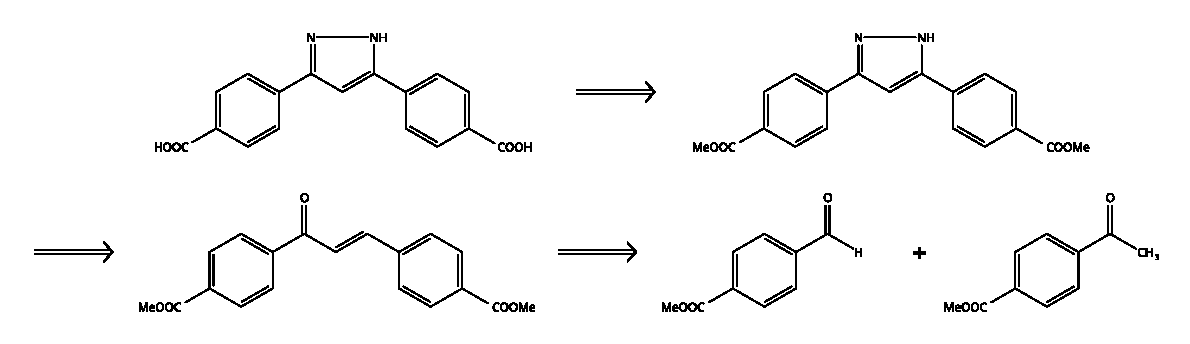
\includegraphics[width=16cm,height=8cm,keepaspectratio]{Structures/pyrazole-retro-alt.eps}
	\caption{Pyrazole Ligand Alternative Retrosynthesis}\label{fig:pyrazole-retro-alt}
\end{figure}

The \(\alpha-\beta\) unsaturated diester intermediate, is asymmetric and carry an olefinic group that should ensure good solubility in less polar organic solvents, allowing to bypass the key problem of solubility encountered with dimethyl 4,4’-malonyldibenzoate.

\subsection{Unsaturaded Diester Formation}\label{sec:alt-pyr-diest}

In order to evaluate the alternative synthetic pathway, with the hope of resolving the series of criticalities encountered, the conditions of formation of the first product reported in the retrosynthesis were evaluated.

\begin{figure}[h!]
	\centering
	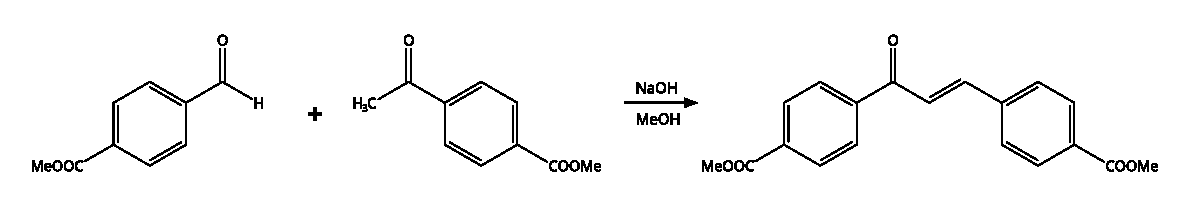
\includegraphics[width=16cm,height=8cm,keepaspectratio]{Structures/unsaturated-synt.eps}
	\caption{Unsaturated Compound Formation}
\end{figure}

The reagents required for the reaction are readily available, and the reaction conditions used follow those classically applied in croton condensation reactions. Some of the variables that can influence the reaction have been analyzed, based on the reagents properties.

\subsubsection{Solvent}

As for the solvent MeOH has been used. It seems the easiest choice to avoid transesterification.\\
Transesterification is the process of converting one ester into another through the exchange of -OR groups. The process requires particular attention under conditions of acidic and basic catalysis at temperatures exceeding room temperature. To prevent this secondary reaction, it is standard in organic chemistry to utilise the alcohol that matches the -OR group to ensure the final product remains unaffected by any substitution.
The potential transesterification products relevant to the discussed reaction are listed below, with the possible substituted ester denoted as R.

\begin{figure}[h!]
	\centering
	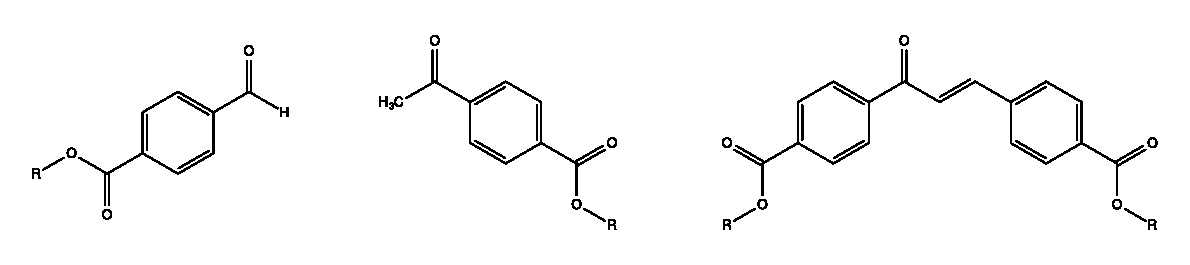
\includegraphics[width=16cm,keepaspectratio]{Structures/esterification.eps}
	\caption{Possibile esterification products}
\end{figure}

Moreover, at the end of the reactions performed, the solvent takes on a yellowish colour that could be associated with the fraction of self-condensation product formed that would then be soluble in MeOH. The condensation product, on the other hand, precipitates quantitatively. This is very useful to avoid any purification steps; any alternative solvent should retain this characteristic.\\
On the basis of the observations, all reactions were carried out in MeOH and the effect of the solvent has not been adequately investigated.

\subsubsection{Reaction Temperature and Reagent Addition}

The ketone could give rise to self-condensation leading to the formation of an unwanted product, reducing the yield and necessitating a purification step. However, the self-condensation reaction is kinetically disadvantageous compared to cross-condensation. For these reasons, a slow addition of the NaOH solution and an ice bath was used.\\
It would also be possible to exploit a slow addition of ketone to a dispersion of NaOH and aldehyde, however this is impractical as the ketone is not soluble in the typical amounts of solvent used and there is a risk of losing some of the reagent in the addition step.\\
Under conditions such as room temperature, 4h reaction time and 1:1 molar ratio of ketone to aldehyde, a yield of 81\% was achieved. This, although satisfactory, can be further optimised.

\subsubsection{Reaction Time}

With regard to the optimal reaction time, some tests were carried out. An increase in reaction time leads to a significant increase in yield without any downside. The results obtained are shown below:

\begin{table}[h!]
	\centering
	\begin{tabular}[b]{cc}
		\toprule
		Time [h] & Yield \\
		\midrule
		4        & 81 \% \\
		15       & 89 \% \\
		\bottomrule
	\end{tabular}
	\caption{Reaction time comparison}\label{tab:hydrazine-ratio}
\end{table}

A longer reaction time leads to a significantly higher yield. Since the reaction takes place at room temperature and there are no special requirements in terms of equipment, there is no reason not to exploit this factor to achieve a higher yield.

\subsubsection{Reagent Proportion}

In order to optimise the reaction yield, it was thought that increasing the ratio of aldehyde to ketone might have a positive effect, as it theoretically reduces the possibility of a self-condensation reaction, given the higher aldehyde ratio.
This possibility was tested with a 1.2 molar ratio of aldehyde to ketone, on an overnight reaction time. The results are shown below.

\begin{table}[h!]
	\centering
	\begin{tabular}[b]{cc}
		\toprule
		Aldehyde Molar Ration & Yield \\
		\midrule
		1                     & 89 \% \\
		1.2                   & 94 \% \\
		\bottomrule
	\end{tabular}
	\caption{Molar ratio comparison}\label{tab:hydrazine-ratio}
\end{table}

It is evident that the effect of the slightly higher ratio is positive, but the effects on the reaction yield of even higher molar ratios have not been investigated: it might be interesting to evaluate this in the future.

\subsection{Hydrazine addition to unsaturated precursor}\label{sec:hyd-add-ins}

\begin{figure}[h!]
	\centering
	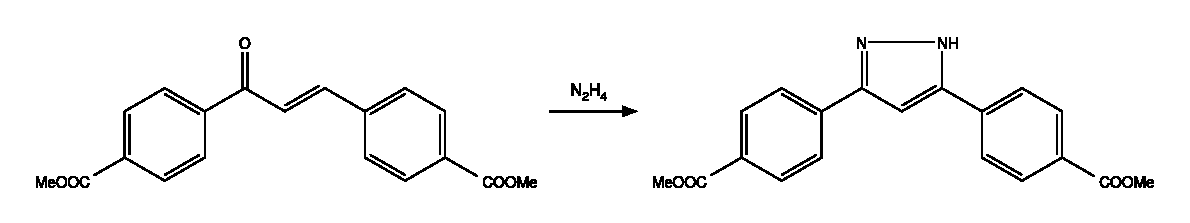
\includegraphics[width=13cm,keepaspectratio]{Structures/pyrazole-form-alternative.eps}
	\caption{Hydrazine reaction with unsaturated compound}
\end{figure}

This step is the crucial one to evaluate the effectiveness of the alternative synthesis, given the difficulties encountered in forming the desired product from diketone.

The reaction mechanism does not differ substantially from that reported for diketone, however several of the difficulties encountered in the previous synthetic pattern, particularly the solubility of the initial compound, should not be encountered in this situation. The mechanism is reported in figure \ref{fig:unsmecha}.
\begin{figure}[h!]
	\centering
	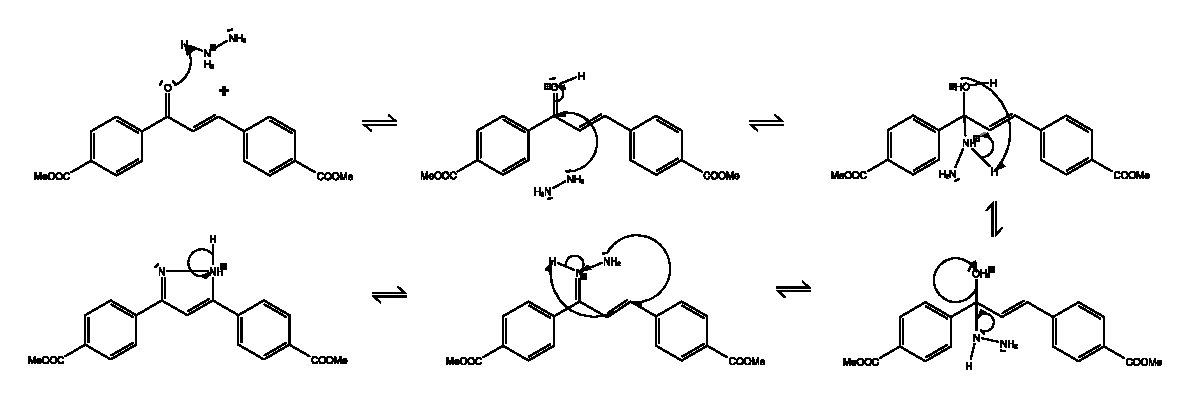
\includegraphics[width=16cm,keepaspectratio]{Structures/unsmecha.eps}
	\caption{Hydrazine coniugate addition mechanism in acid condition}\label{fig:unsmecha}
\end{figure}
\newpage

The conditions and results obtained for the formation of the pyrazole ring are evaluated, which include different solvents, catalysts, reaction times and the use of the microwave reactor. The conditions used were chosen from those reported in the literature \cite{leavai_synthesis_2002}, verifying the effectiveness of each procedure and modifying what was reported as needed.

\subsubsection{Acetic Acid}\label{sec:ace-cond}

According to the article in the literature, this synthetic route should be the simplest and most effective one, capable of achieving high reaction yields.\\ The reaction is conducted in acetic acid in the presence of hydrazine, with temperatures and reaction times that may vary depending on the substrate. At the end of the reaction, the product should precipitate spontaneously, and the same should be easily recoverable by filtration.

However, on a practical level it was not optimal and the results obtained are discouraging. Neither product nor intermediate formation was observed, which reportedly should have been possible to isolate. No effects were observed even by extending reaction times and raising temperatures. The obtained results are reported below and the detailed experimental information are in the chapter\ \ref{cha:experimental-section}.

\begin{table}[h!]
	\centering
	\begin{tabular}[b]{cccc}
		\toprule
		ID & Temperature [K] & Time [h] & Yield \\
		\midrule
		A  & RT              & 1        & -     \\
		B  & 363             & 3        & -     \\
		C  & 393             & 48       & -     \\
		\bottomrule
	\end{tabular}
	\caption{Acetic acid reaction yields}\label{tab:hydrazine-ratio}
\end{table}

The results obtained did not meet expectations; although the reagent dissolved easily at higher temperatures than in test B, no product was recovered.
In addition, investigation of the composition of the mixture were made difficult by the large amount of acetic acid present. Cooling the mixture succeeded in observing extensive precipitation of what was later identified with difficulty as the initial reagent.

\subsubsection{Methanol with acid and basic catalysis}\label{sec:et-ac-bas}

In addition to the conditions used with acetic acid, which proved to be a failure with this initial reagent, conditions including the use of methanol as a solvent in the presence of acidic and basic catalysts, such as hydrochloric acid and pyridine, are reported in the literature.

In relation to the use of hydrochloric acid as a catalyst the results obtained are poor. The addition of hydrazine to the solution of hydrochloric acid in methanol causes a rather violent reaction, subsequently the initial reactant does not solubilize. In the reaction time no change is observed. No product formation is observed, and the mixture does not develop blue photoluminescence. These reaction conditions were then not further investigated.

Unlike what is found in conditions of acid catalysis, the use of pyridine as a catalyst initially seems to lead to better results.
The initial reactant completely solubilized, and the mixture was left to react under reflux.

\subsubsection{Ethanol}\label{sec:met-only}

As a result of the difficulties encountered previously, several tests were carried out in ethanol alone, at varying temperatures and reaction times, maintaining the molar ratio costant.

The progress of the reaction was checked at room temperature, in the presence of 3 moles of hydrazine per moles of initial reagent, overnight, under strong stirring. The formation of crystalline product, with blue photolumiscence, was observed. What apparently looked like it might be the desired product, upon coupled NMR analysis such as COSY and NOESY turned out to be the hydrazonic intermediate whose structure is given below.

\begin{figure}[h!]
	\centering
	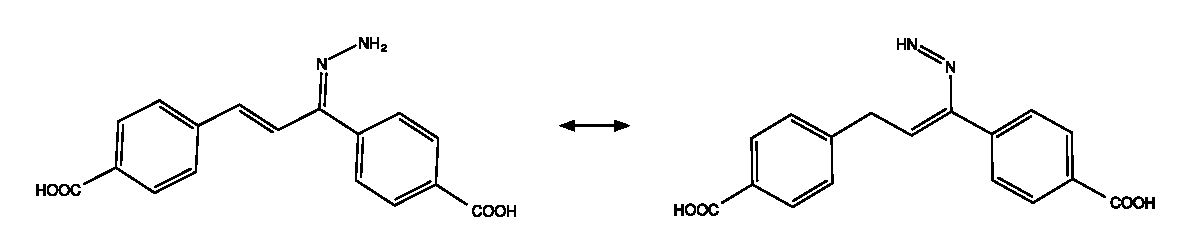
\includegraphics[width=13cm,keepaspectratio]{Structures/idrazone.eps}
	\caption{Intermediate compound structure}
\end{figure}

Indeed, within the literature it was reported that the intermediate could be obtained without proceeding to pyrazole ring closure. By raising the temperature, which should have a positive effect in this case, no change was observed in the product formed despite several hours of reaction. However, the crystallinity of the precipitate formed appears to the eye to be of a higher degree. The structure of the compound identified as an intermediate was again identified using NMR (\ref{ap:intermediate}).

\begin{figure}[h!]
	\centering
	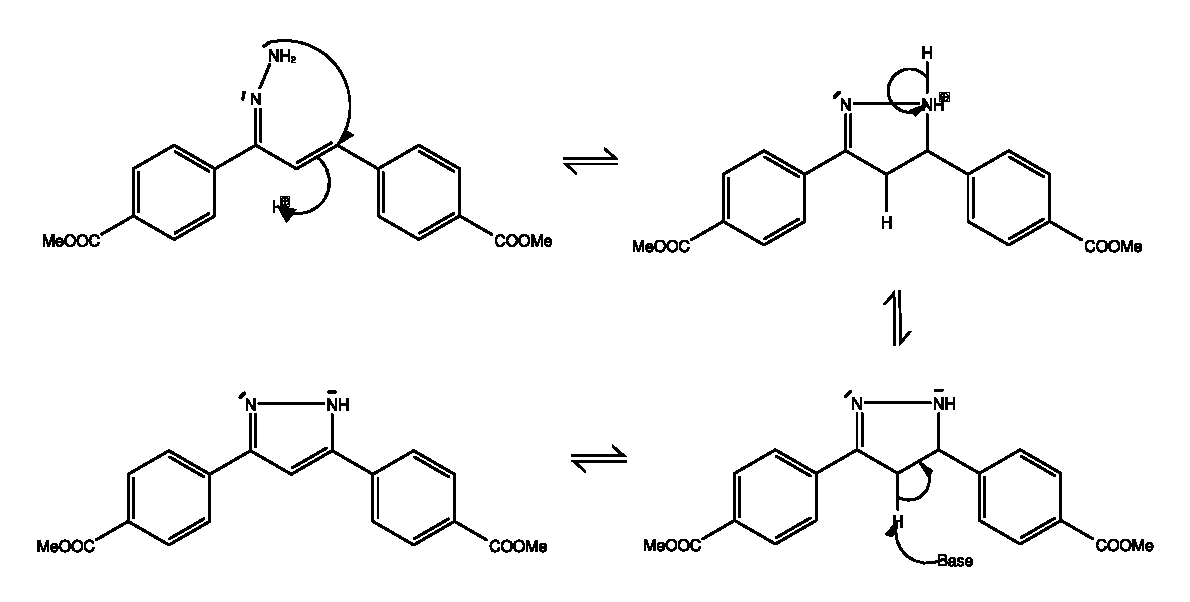
\includegraphics[width=11cm,keepaspectratio]{Structures/idrazonemecha.eps}
	\caption{Idrazone intermediate mechanism toward pyrazole formation}
\end{figure}

\subsubsection{Microwaves}\label{sec:micro}

Microwave reactors have emerged as powerful tools in the field of chemistry \cite{priecel_advantages_2019}, offering numerous advantages over traditional heating methods.

\begin{figure}[h!]
	\centering
	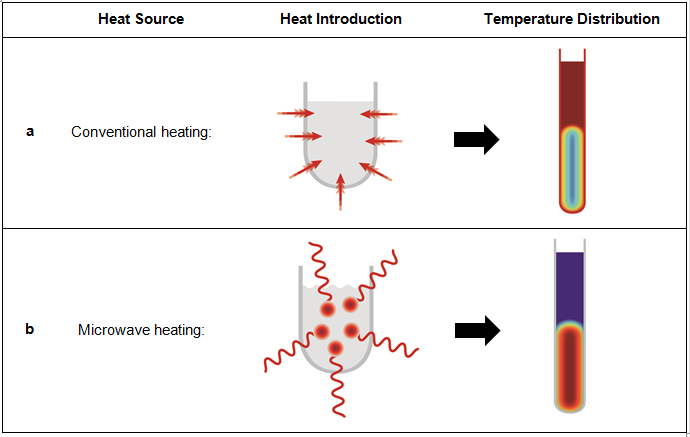
\includegraphics[width=8cm,keepaspectratio]{Images/05_microwave-heat-introduction.jpg}
	\caption{A good representation of the fundamental difference between traditional heating methods and microwaves, where the heat actually comes from the ``inside''.}
\end{figure}

They are able to heat reaction mixtures very quickly, promoting mixing. They also provide granular control of temperature curves and easily allow working at pressures above atmospheric, reaching temperatures above the boiling temperature of the solvent itself at SATP. The amount of solvent used is small, it is not challenging to run reactions with small amounts, and the whole process is energy efficient.

Especially with regard to cyclization reactions and the formation of pyrazolines, several examples are available in the literature \cite{azarifar_microwave-assisted_2003}. The high temperature and pressure make the reactions more selective by providing higher yields; in addition, reaction times are greatly reduced from hours to tens of minutes.

The experiment carried out was primarily exploratory in terms of the reaction tested. Two heating cycles were conducted at 500 W for 10 minutes under conditions that have been studied in the literature and are comparable to those in acetic acid as reported in section\ \ref{sec:ace-cond}, starting from the idrazone intermediate obtained before.\\
No product formation was observed, and the reaction mixture remained in an unprecedented state. Additional research is necessary to fully assess the by-products generated.
To draw accurate conclusions and thoroughly analyse the impact of microwave application, it is imperative to conduct systematic tests. These tests should analyse the effect of elevated temperatures and, in particular, pressure.

\subsection{Pyrazole Ester Hydrolisis}\label{sec:pyrazole-hydro}

\begin{figure}[h!]
	\centering
	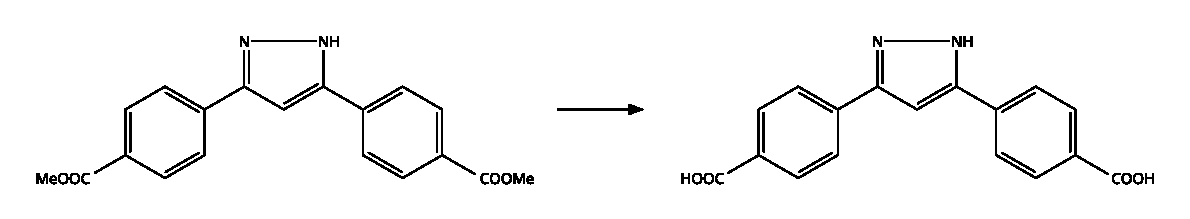
\includegraphics[width=13cm,height=8cm,keepaspectratio]{Structures/pyrazole-hydro.eps}
	\caption{Pyrazole Diester Hydrolisis}\label{fig:pyrazole-form}
\end{figure}

The removal of methyl esters is a standard practice in organic chemistry, and no specific problems were encountered during this step of the synthesis. Two synthetic routes were analyzed.
Initially, removal with LiOH in THF:H$_2$O 1:1 was used, but the yields of the different reactions were not highly reproducible, perhaps because of the precariousness of the different impurities resulting from the different methods of pyrazole synthesis. \\
Instead, removal with NaOH in MeOH:H$_{2}$O 1:1 could give better results, with higher yield and cleaner processing. This method has not been properly evaluated.

The tests carried out yielded only a few tens of milligrams of acid from less than a hundred milligrams of starting ester. The ester subjected to hydrolysis was always derived from different syntheses and processes, and the appearance of the reaction mixture always varied slightly in colour and behaviour, especially with regard to the pH at which the small product formed began to precipitate.
The data for this reaction cannot be reliably summarised.Thus, this aspect of the synthesis will have to be finalized when the ester synthesis is optimised.

\subsection{Conclusions, considerations and further development}

Due to the extensive number of trials conducted, the initially reaction path, which included the option of acquiring the required product from DikDiEst, cannot be deemed feasible. Whilst the cross-Claisen reaction allows for the acquisition of the crucial intermediate for the direct addition of hydrazine, the latter step is currently infeasible as the yields are not satisfactory to ensure the possibility of exploring the reactivity of the binder in question.\\
However, the challenges faced during this stage have highlighted significant factors that must be considered to avoid prospective obstacles. Notably, solubility has been identified as a vital component to enable the modification and variation of previously examined ligands, which can also pose a demanding and resource-intensive undertaking.

Despite some challenges encountered during this initial experience, the alternative synthetic pattern has shown promising results. In comparison to the cross Claisen of the initial pattern, the mixed aldolic condensation is faster and easier to perform, enabling us to evaluate numerous conditions related to the conjugated addition of hydrazine. Nevertheless, we still faced several criticalities during the latter step. The findings generated elicit a stronger hope than the prior approach, consideration, and further investigation.\\
Microwave reactors could be the optimal approach for cyclization reactions of this sort, including routine production of ligands, given its suitability and potential for agile scaling.
Microwave reactors are potentially the optimal route for cyclization reactions of this kind, as well as for routine ligand production due to their ability to facilitate agile scaling.
Future investigation could explore the response to a mechano-chemical reaction, which is conducted in the solid state and may prove an interesting topic.

As for the hydrolysis reaction, this can only be investigated and consequently optimized following an effective method of obtaining it in the ester intermediate. This aspect, too, will have to be investigated and taken care of in future developments in order to obtain the binder in considerable quantities.

\newpage
If the aforementioned alternatives prove unviable or do not yield the desired outcome, one may opt for a cross-coupling reaction like rsuzuki to acquire the ligand. Nevertheless, procuring the necessary reagents in substantial quantities akin to those utilized in prior experiments may prove challenging.

\begin{figure}[h!]
	\centering
	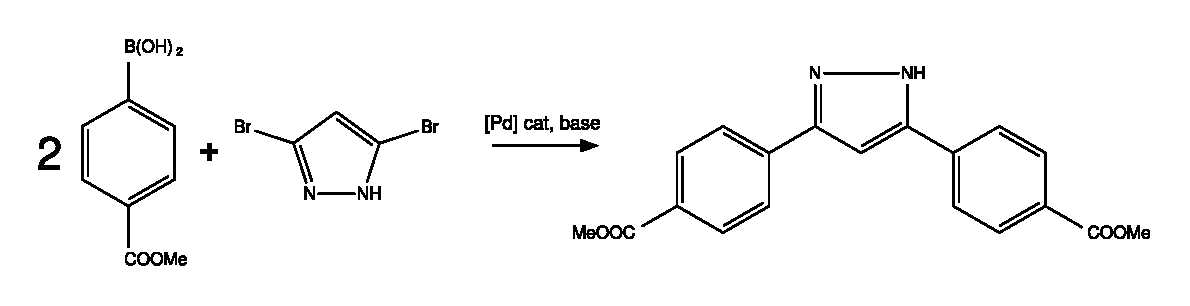
\includegraphics[width=14cm,height=8cm,keepaspectratio]{Structures/suzuki.eps}
	\caption{Hypothesis of suzuki coupling-reaction}
\end{figure}

\newpage
\section{Electrochemistry}\label{sec:electrochemistry}

\subsection{Why electrochemistry and cyclic voltammetry?}\label{sec:elect-intro}

Cyclic voltammetry (CV) is a technique used in the analysis of organic and inorganic compounds\ \cite{elgrishi_practical_2018}. It provides information about reduction and oxidation processes of molecular species, the stability, the conversion and storage of energy and several other interesting properties. CV is also invaluable to study electron transfer-initiated chemical reactions, which includes catalysis. CV can be used to estimate the electron affinity and ionization energy of test compounds in a much cheaper and faster way compared to other high vacuum methods. It is important in electrochemistry because it allows to study the electron transfer processes that are at the center of the reactivity of inorganic complexes.
The aforementioned parameters correlate with the energy levels of highest occupied molecular orbital (HOMO) and lowest unoccupied molecular orbital (LUMO).

When cyclic voltammetry (CV) is combined with or ultraviolet-visible and near-infrared (UV-Vis-NIR) spectroscopies, it provides useful information such as electron affinity, ionization potential, band-gap energies, the type of charge carriers, and degradation information\ \cite{pluczyk_using_2018}. Analizing the CV experiment data is possible to determine the band-gap value that can be later evaluted against the one obtained from the spectroscopic UV data.

\subsection{Ligands and Background}

Electrochemistry exploration has been carried out on already studied and synthetized compounds\ \cite{carlucci_heterometallic_2010}. In the following section, the properties and peculiarities of the ligands and the monomers and MOFs connected to them will be outlined, with the intention of clarifying the significance of the corresponding electrochemical investigation.

Detailed synthesis of ligand, monomers and MOFs are given in chapter\ \ref{cha:experimental-section}.

In the following section, the properties and idiosyncrasies of the ligands and the monomers and MOFs connected to them will be outlined, with the intention of clarifying the significance of the corresponding electrochemical investigation.

Previous research aimed to develop a modular system of tris-chelate metalloligands using the DikDiCN ligand.
% See the summary shown in the figure for more details.
This approach utilizes 6 nitrile groups to facilitate the utilization of metalloligands as building blocks to construct networks with silver centers.

\begin{figure}[h!]
	\centering
	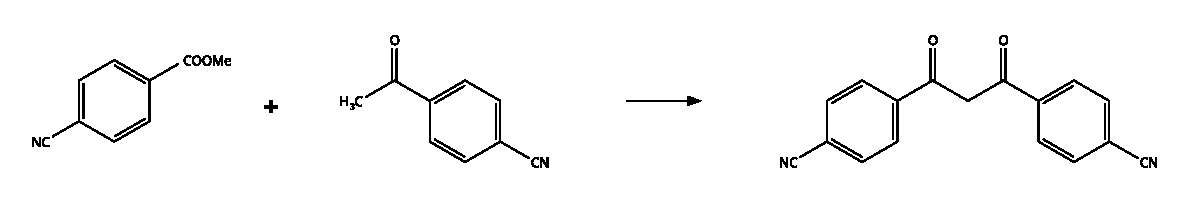
\includegraphics[width=16cm,height=8cm,keepaspectratio]{Structures/dicn-sint.eps}\caption{DikDiCN synthesis}
\end{figure}

The ligand reacts with different metal salts, resulting in the creation of monomers. These monomers are grouped into families based on the oxidation state of the central metal.

\begin{figure}[h!]
	\centering
	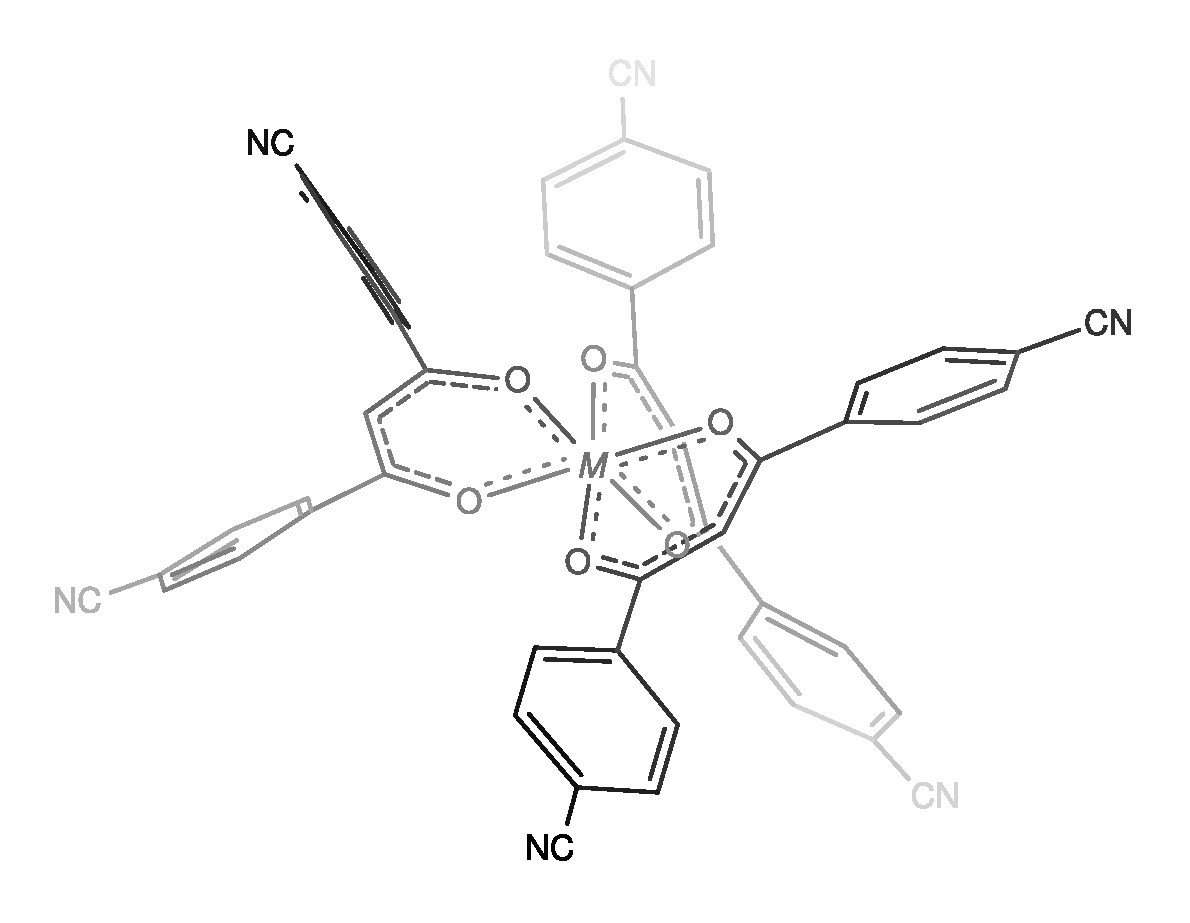
\includegraphics[width=10cm,keepaspectratio]{Structures/monomero.eps}\caption{Rappresentative metalloligand structure}
\end{figure}
\newpage

The reaction of two types of metalloligands \([M^{III}L_{3}]\) and \([M^{III}L_{3}]^{-}\) with different silver salts led to the preparation of two families of MOFs. The aforementioned contains a positively charged ion such as \([Et_{4}N]^{+}\) within the crystal structure's pores, thus ensuring neutrality.\\
Metalloligands of Fe (III), Co (III), Mn (II), Co (II), Zn (II), and Cd (II) have been prepared successfully.
It should be noted that not all have been successfully synthesized until the corresponding Metal-Organic Frameworks (MOFs) were formed. A table displaying the obtained species is included.\\

\begin{table}[h]
	\centering
	\begin{tabular}{cc}
		\toprule
		Metalloligand central metal & Ag counter ion                                                                                                 \\
		\midrule
		Fe III                      & \(CF_{3}SO_{3}^{-},\ PF_{6}^{-},\ BF_{4}^{-},\ ClO_{4}^{-}\)                                                   \\
		Co III                      & \(CF_{3}SO_{3}^{-},\ BF_{4}^{-},\ SbF_{6}^{-}\)                                                                \\
		Mn II                       & \(BF_{4}^{-}\)                                                                                                 \\
		Zn II                       & \(CF_{3}SO_{3}^{-},\ PF_{6}^{-},\ BF_{4}^{-},\ ClO_{4}^{-}, AsF_{6}^{-},\ SbF_{6}^{-},\ NO_{3}^{-},\ TsO^{-}\) \\
		Cd II                       & \(BF_{4}^{-},\ ClO_{4}^{-}\)                                                                                   \\
		\bottomrule
	\end{tabular}
	\caption{Obtained MOFs from metalloligands}
\end{table}

Remarkably, all of these species maintain identical crystal structures and crystallize in a trigonal space with notably similar cell parameters, despite variations in central metals, ionic charges, and silver-derived counter anions.\\
Additionally, the species' crystallization results in the creation of a net interpenetrating structure, with each possessing a distinct chirality (\(\Delta\) and \(\Lambda\)).
The structure contains hexagonal channels accounting for approximately 40\% of the cell volume, allowing for the reversible removal of solvent molecules. It can also conduct anion exchange in single-crystal to single-crystal processes.

\subsection{Electrochemical interest}

The electrochemical significance of the prior research is multifaceted.\\
Primarily, the ligand accommodates two active redox groups, specifically the nitrile groups and there are numerous other similar ligands based on diketones available from previous studies. This enables a comparative study of the electrochemical reactivity within the ligand family.\\
The analysis of the electrochemical activity of monomers can verify the effect of coordination on the groups present. This can be achieved through examining the function of various metals with which the ligand forms monomers. Despite varying metals, the structure of the trichelate remains constant.\\
The MOFs resulting from the reaction of metalloligands with silver salts are highly noteworthy from an electrochemical perspective since, as previously mentioned, the structures  remain intact even as the metal and any counterions undergo modification.

\subsection{Ligands set}

The electrochemical properties of a ligand systematic series, all of them CN-terminated (Figure \ref{fig:lig-set}). \\

\begin{figure}[h!]
	\centering
	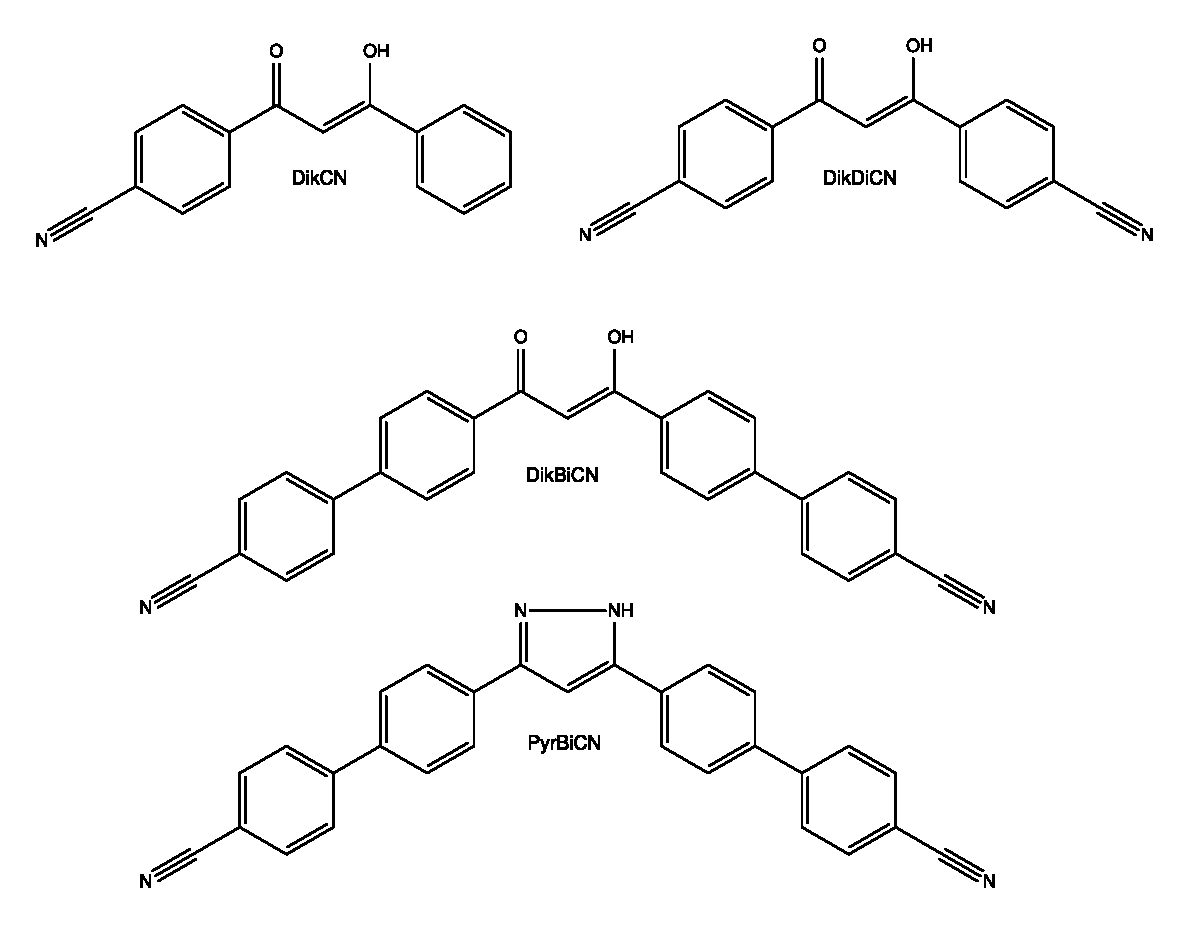
\includegraphics[width=10cm,keepaspectratio]{Structures/mussini/leganti.eps}
	\caption{Ligand set}
	\label{fig:lig-set}
\end{figure}

Additional ligands currently under investigation for other projects are being scrutinised in addition to those already discussed in prior sections.
All the ligands have been investigated by cyclic voltammetry CV in a wide potential scan rate range (and by differential pulse voltammetry DPV, too), in \(CH_{3}CN\) (in one case also in \(CH_{2}Cl_{2}\)) with 0.1 M tetrabutylammonium hexafluorophosphate, \(TBPF_{6}\) as supporting electrolyte, in a three-electrode minicell (working solution volume = 3 \(cm^{3}\)), including:

\begin{itemize}
	\item a glassy carbon GC disk electrode (AMEL, geometric surface \(\simeq\) 0.071 \(cm^{2}\)); the electrode surface can be reproducibly cleaned when needed by mechanical treatment with synthetic diamond powder (Aldrich) on a wet cloth (Struers DP-Nap, usually employed for preparation of metal samples) followed by rinsing with deionized water and drying by wiping with porous paper;
	\item a platinum wire counter electrode;
	\item a saturated calomel electrode (SCE) as reference electrode, inserted in a glass compartment provided with a porous frit, filled with the working solvent + supporting electrolyte medium, to prevent water and chloride leakage into the working electrode compartment. The potentials were afterwards referred to the formal potential \(E ^{\circ}’\) of the ferricinium\vert ferrocene (\(Fc^{+}|Fc\)) chemically and electrochemically reversible redox couple, measured  vs the operating SCE reference electrode in the same session and in the same conditions, as the average between forward and backward ferrocene CV peak potential); in fact, according to IUPAC\ \cite{gritzner_recommendations_1982} the energetics of the ferrocene couple can be assumed as (approximately) invariant with solvent, and therefore it is usually adopted as intersolvental potential reference, enabling to normalize measurements in different media by elimination of the intersolvental liquid junction potential between the saturated KCl solution of the reference electrode and the working solution. Only after such normalization one can properly evaluate possible solvent effects on the investigated electron transfer process.
\end{itemize}

The measurements were performed using an Autolab potentiostat managed by a PC with GPES software, also enabling to compensate the ohmic drop by the positive feedback method\ \cite{bard_electrochemical_2001}.
A synopsis of selected CV patterns recorded at 0.2 \(V/s\) is provided in the figure \ref{fig:synops}, in which currents have been normalized by geometric surface, ligand concentration and square root of potential scan rate (\(I/(Scv^{0.5})\)) [\(A cm^{-2} mol^{-1} dm^{3} V^{-0.5} s^{0.5}\)], and potentials have been normalized vs the Fc+|Fc couple as above mentioned.

\begin{figure}[h!]
	\centering
	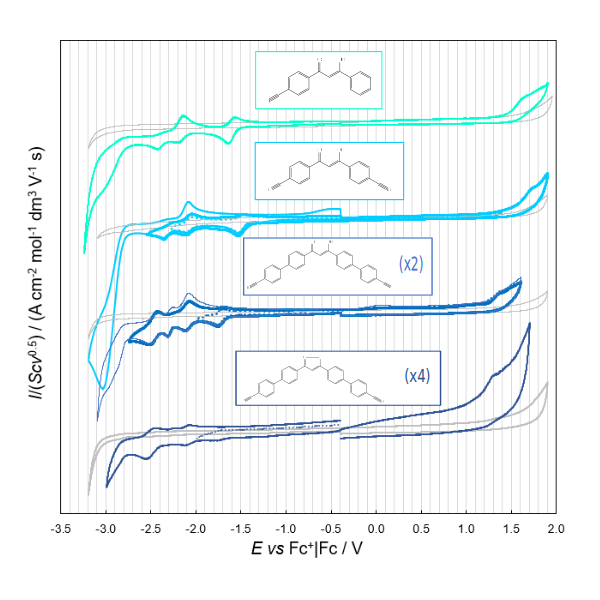
\includegraphics[width=10cm,keepaspectratio]{Images/mussini/secondaimmagine.pdf}
	\caption{CV pattern synopsis}
	\label{fig:synops}

\end{figure}
\newpage

As a very preliminary discussion (a more detailed examination is planned on the
many acquired CV and DPV data) it can be noticed that in all cases the CV
patterns are consistent with the electron poor character of the ligands on
account of their electron attracting -CN and -C=OR substituents (0.66 and \simeq 0.5
\(\sigma p\) \ Hammett constants respectively\ \cite{hansch_survey_1991}). In particular:
\begin{itemize}
	\item only one oxidation process is observable, close to the oxidative background;
	\item instead a series of subsequent reduction events appear in the available potential window, starting at relatively mild potentials, some of them tending to reversibility from the electrochemical point of view (fast electron transfer with negligible activation barrier, accounted for by the peak potentials being nearly unaffected by the scan rate) and/or from the chemical point of view (rather stable electron transfer product accounted for by the presence of a return peak increasingly symmetrical with increasing scan rate).
\end{itemize}

For a very preliminary discussion it is convenient to start with the symmetrical DikDiCN case as the ligand series benchmark. Actually, considering the keto-enol tautomerism on the ligand core, DikDiCN might be expected to correspond to a case of two equivalent, reciprocally interacting redox sites, which usually result in a system of two, reciprocally connected, subsequent CV peaks of similar features, their distance accounting for the reciprocal interaction between the equivalent redox sites. This might apply to the first two DikDiCN reduction peaks observed in our CV patterns; however, any conclusion should wait for the planned more exhaustive data examination, since the reductive CV pattern includes more than two peaks, only partially reversible at low/medium scan rate, with formation of some oxidizable products on the electrode surface being observed as a consequence of the reduction events upon repeated potential cycling.

Comparing DikDiCN with DikCN or DikBiCN enables to make a preliminary evaluation of inductive and conjugation effects. It is worthwhile recalling that

\begin{itemize}
	\item In a systematic series of aromatic/polyconjugated molecules, substituent inductive effects typically result in potential shifts for both first oxidation and first reduction in the same direction (in particular, in positive direction with increasingly electron attracting substituents, making reductions easier but oxidations more difficult, and vice versa in negative direction with increasingly electron donating substituents). Concerning the shift magnitude, (i) it decreases with increasing distance between substituent and redox site; (ii) it is comparable for first oxidation and reduction processes if they involve the same redox site, while it can be significantly different if the two processes are located on different redox sites.
	\item Radical anion and radical cation formation, i.e. the usual first reductive and oxidative electron transfer processes in a polyaromatic system, are both favoured by an increase in conjugation; thus increasing conjugation efficiency results in both milder oxidation potentials and milder reduction potentials (unlike inductive effects).
\end{itemize}

Now, asymmetrical DikCN exhibits a CV pattern very similar to the DikDiCN one, but shifted (at least concerning the first and third reduction peaks and the first oxidation peak) by approximately 0.1 V towards more negative/less positive potentials; this is consistent with its featuring only one nitrile group, resulting in a globally lower electron attracting inductive effect, which makes the reduction processes more difficult and the oxidation process easier. A further difference respect to DikDiCN is the decrease in the formation of products on the electrode surface as a consequence of the reduction processes.

Even more conspicuous are the negative shifts of both oxidative and reductive CV peaks of DikBiCN respect to benchmark DikDiCN; and notably, in this case the shifts are of different magnitude although in the same direction; in particular, the shift is more conspicuous for the oxidation process. Possibly, in the biphenyl case on one hand the increase in conjugation efficiency should be only a moderate one on account of the torsional angle between the two phenyl rings, on the other hand the CN and C=O electron attracting substituents would be placed on two different, only partially conjugated aromatic rings, instead than on the same ring; maybe such “dilution” of the inductive effects could prevail on the slight increase of the overall conjugation. In any case, the different magnitudes of the first oxidation and first reduction potential shifts could point to the two processes involving significantly different redox sites (maybe, the reduction one closer to the CN terminals and the oxidation one closer to the core.

The CV patterns recorded for PyrBiCN appear similar (maybe too similar?) to the parent DikBiCN case, but their discussion is difficult since they look much smaller and less defined respect to former cases (in the figure they have been multiplied by a 4 factor respect to DikDiCN). We look forward to performing a check on the sample nature and purity before repeating the CV investigation.

It is worthwhile mentioning that possibly in the DikDiCN and DikBiCN cases the low solubility can be responsible of the lower observed current intensity. However, better resolution might be obtained by analysis of DPV data.

In the case of DikDiCN we also recorded in \(CH_{2}Cl_{2}\) + 0.1 M \(TBAPF_{6}\) the ligand pattern as well as the pattern of its nominal \(Fe(III)(DikDiCN)_{3}\) complex.  As shown in Figure \ref{fig:CVDikDICN} the solvent effect on the electrochemical properties of the ligand after duly normalizing the CV patterns vs the Fc couple only looks a slight one. Of course the \(CH_{2}Cl_{2}\) window is narrower on the reduction side respect to the \(CH_{3}CN\) one on account of the solvent undergoing reduction at much milder potentials; thus the fourth DikDiCN reduction peak is not perceivable in \(CH_{2}Cl_{2}\).

\begin{figure}[h!]
	\centering
	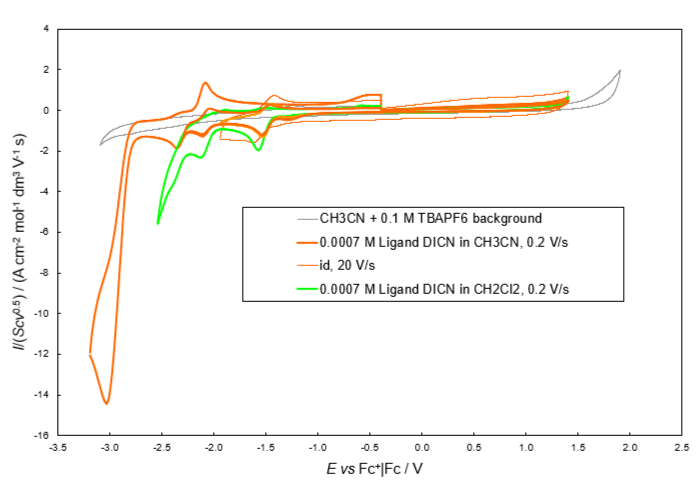
\includegraphics[width=8cm,keepaspectratio]{Images/mussini/penultimafigura.pdf}
	\caption{CV of DikDICN in \(CH_{2}Cl_{2}\)  and \(CH_{3}CN\)}\label{fig:CVDikDICN}
\end{figure}
\newpage

\subsection{Monomer and MOFs sets}\label{sec:mofmon}

Initial testing was conducted on the synthetized monomers, revealing the notable existence of ligand residues. In order to carry out electrochemical measurements, it is essential to purify the products, which is planned as a future undertaking following further analysis.

In particular, \([ Fe^{III}(DikDiCN)_{3} ]\) investigation is reported: its CV pattern looked nearly identical to the free ligand (Figure \ref{fig:feCV}).

\begin{figure}[h!]
	\centering
	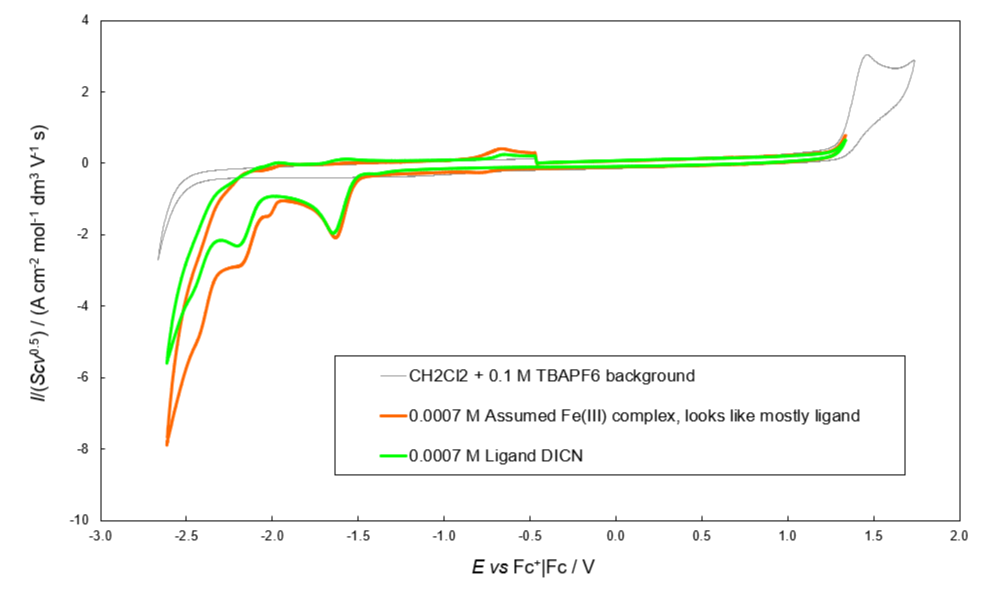
\includegraphics[width=10cm,keepaspectratio]{Images/mussini/ultimafigura.pdf}
	\caption{Monomer and DikDiCN comparison}\label{fig:feCV}
\end{figure}


For MOFs measurements, the material must be deposited on an electrode in ITO (Indium Tin Oxide). While exploratory tests have been carried out, there is a need for adequate investigation of the deposition procedure and subsequent analysis in the future.

\subsection{Conclusions, considerations and further development}

The research carried out on the electrochemical aspect of these structures in significally interesting both for electrochemists and inorganic chemists. However, to gain a better understanding of the initial observations, further in-depth analyses of the ligands, particularly the monomers and MOFs, are necessary.
The objective of this section is to compare several series of ligands, monomers and MOFs to identify structural trends within a specific family. Therefore, in order to expand the range of structures, it would be beneficial to synthesise ligands similar to those used in this study.
\end{document}

%%% Local Variables:
%%% mode: latex
%%% TeX-master: "../Master"
%%% End:


